% =============================================================================
%  Group 10 -- final report, Deep Learning for Visual Recognition (AU, 2026)
%  SCAFFOLD. Grey boxes = points to make, in order, with the numbers to use.
%  Replace each grey box with your own prose, then delete the box.
%  Tables and figures are final (built by make_figures.py from results/).
%  Budget: 6--8 pages incl. figures, ~3,800 words (style guide, 3 Nov).
%  Build:  cd report && latexmk -pdf main.tex
% =============================================================================
\documentclass{article}
\usepackage{arxiv}
\usepackage[utf8]{inputenc}
\usepackage[T1]{fontenc}
\usepackage{hyperref}
\usepackage{url}
\usepackage{booktabs}
\usepackage{amsmath,amssymb}
\usepackage{graphicx}
\usepackage[numbers,sort&compress]{natbib}
\usepackage{xcolor}
\usepackage{enumitem}
\usepackage{caption}
\captionsetup{font=small,labelfont=bf}

% ---- scaffold helpers (delete with the last grey box) -----------------------
\definecolor{notebg}{HTML}{F2F1EE}
\definecolor{noteink}{HTML}{52514E}
\newenvironment{notes}[1][]{%
  \par\smallskip\noindent\color{noteink}\small
  \textbf{[Points to make\if\relax\detokenize{#1}\relax\else\ --- #1\fi]}
  \begin{itemize}[leftmargin=1.2em,itemsep=1pt,topsep=1pt]}
  {\end{itemize}\normalsize\color{black}\smallskip}
% -----------------------------------------------------------------------------

\renewcommand{\headeright}{DLVR 2026 -- Group 10}
\renewcommand{\undertitle}{Course project report}
\renewcommand{\shorttitle}{Class imbalance in melanoma classification}

\title{Do class-imbalance treatments help a network detect melanoma?\\
\large A controlled study on ISIC 2020}

\author{Luan Ramm \And David Kaznelson \And Mikkel Lassen \\
Aarhus University}
\date{December 2026}

\begin{document}
\maketitle

% =============================================================================
\begin{abstract}
\begin{notes}[150--180 words; write it last]
  \item Context, one sentence: melanoma detection from dermoscopy; in ISIC 2020 only 1.8\% of 33,126 images are melanoma.
  \item Question: do imbalance treatments (weighted loss, balanced sampling, focal loss, AUC-margin loss) make the network \emph{separate} melanoma from benign lesions better, or only move the decision threshold?
  \item Method: ResNet-18, two fine-tuning depths, 5 patient-grouped folds, AUPRC as the main metric, rules fixed in advance; then an extension that changes the data and the backbone.
  \item Finding 1: weighted loss, balanced sampling and focal loss did not beat plain BCE (fold AUPRC 0.149--0.165 vs 0.159); they move the threshold and worsen calibration. Only the AUC-margin loss gained, slightly (0.169; test 0.187 vs 0.154).
  \item Finding 2 (headline number vs baseline): a fine-tuned dermatology foundation model (PanDerm) trained with extra ISIC 2019 melanomas reached AUPRC \textbf{0.291} (95\% CI 0.197--0.394) on the locked test set against \textbf{0.154} for plain BCE; at the same threshold rule it found 87\% of melanomas with 44\% fewer false alarms.
  \item Conclusion, one sentence: the bottleneck is how much the network knows about melanoma, not how the loss weighs the classes.
\end{notes}
\end{abstract}

\keywords{Melanoma \and class imbalance \and focal loss \and calibration \and foundation models \and ISIC 2020}

% =============================================================================
\section{Introduction}
\label{sec:intro}
\begin{notes}[300--400 words, no subsections]
  \item Problem: melanoma is the deadliest skin cancer; early detection matters; CNNs reach dermatologist-level accuracy on curated data~\cite{esteva2017dermatologist}.
  \item What makes it hard: in screening data almost every lesion is benign. ISIC 2020~\cite{rotemberg2021patient}: 584 melanomas in 33,126 images (1.8\%), about 55 benign lesions per melanoma. A network trained with plain cross-entropy then gives almost every image a low score: at threshold 0.5 our baseline finds 7 of 499 melanomas.
  \item The usual remedies: re-weight the loss, re-sample the data, or change the loss (focal loss). Gap: these mainly change \emph{where} the 0.5 threshold falls, which can also be done after training for free. Whether they also improve how well the network separates the two classes is rarely tested separately (Kang et al.~\cite{kang2020decoupling} for long-tailed classification).
  \item \textbf{State the research question as its own sentence, in italics:} \emph{Do class-imbalance treatments make a network separate melanoma from benign lesions better, or do they only move the decision threshold?}
  \item Approach in one sentence: four treatments vs plain BCE on the same ResNet-18, two fine-tuning depths, 5 patient-grouped folds, threshold-free metric (AUPRC), decision rules written down before the runs; then an extension that changes what the network knows (images, backbone, extra data); a locked test set opened once.
  \item Contributions, numbered list of 3: (1) a controlled comparison showing that the treatments move the threshold but do not improve separation, and cost calibration; (2) evidence that the limit is the number of melanomas and the features, not the loss: extra ISIC 2019 melanomas and a dermatology foundation model improve separation, together nearly doubling AUPRC; (3) a test of how to choose the threshold (``find 80\% of melanomas'' transfers, ``best F1'' does not).
\end{notes}

% =============================================================================
\section{Related work}
\label{sec:related}
\begin{notes}[350--450 words; for each paper: what they did, their result, and one sentence ``like / unlike them, we \ldots'']
  \item \textbf{Dataset:} Rotemberg et al.~\cite{rotemberg2021patient} released ISIC 2020 with patient ids so that lesions of one patient can be compared. We use the patient ids to keep a patient's images in one fold.
  \item \textbf{Imbalance in CNNs:} Buda et al.~\cite{buda2018systematic} found oversampling the most effective remedy on artificially imbalanced image sets, and that a threshold shift should accompany it. Kang et al.~\cite{kang2020decoupling} showed that in long-tailed recognition, re-balancing mainly helps the classifier layer, not the learned features. Our grid tests both claims on real, naturally imbalanced medical data, at two depths.
  \item \textbf{Focal loss and calibration:} Lin et al.~\cite{lin2017focal} introduced focal loss for dense detection (1:1000 foreground/background). Mukhoti et al.~\cite{mukhoti2020calibrating} found it \emph{improves} calibration of over-confident networks. Unlike their setting, our BCE baseline is already well calibrated (ECE 0.006), and focal loss makes calibration worse (0.091).
  \item \textbf{Optimising the ranking directly:} Yuan et al.~\cite{yuan2021large} proposed the AUC-margin loss (LibAUC) and placed in the top 1\% of the ISIC 2020 challenge with it. We use it as a fourth treatment (E6).
  \item \textbf{ISIC 2020 winners:} Ha et al.~\cite{ha2020identifying} won with an ensemble of EfficientNets on large images, ISIC 2019 as extra training data and patient metadata. We test three of these ingredients one at a time on a single small network, not to compete with their ensemble.
  \item \textbf{Dermatology foundation model:} Yan et al.~\cite{yan2025panderm} pretrained PanDerm, a ViT-B/L, self-supervised on about 2 million skin images, and report strong linear-probe results. We test it frozen and fine-tuned, and check for overlap between its pretraining data and our test set.
  \item Optional, one line: Kurtansky et al.~\cite{kurtansky2024patient} found that patient context (the ``ugly duckling'' sign) did not improve AI or readers in the challenge, which is why we did not pursue it. (CHECK the reference before hand-in.)
\end{notes}

% =============================================================================
\section{Methods}
\label{sec:methods}

\subsection{Data and splits}
\begin{notes}[~200 words]
  \item ISIC 2020 training set, 256$\times$256 JPEGs (C.~Deotte's resized version on Kaggle). After removing the organisers' 425 duplicate pairs: 32,693 images.
  \item Locked test set: 4,630 images (82 melanomas, 309 patients), split off once on 22 Sep, opened once on 4 Nov.
  \item Development set: 28,063 images (499 melanomas, 1,747 patients) in 5 patient-grouped, label-stratified folds (94, 84, 99, 128, 94 melanomas). Each run trains on 4 folds and is scored on the 5th (the held-out fold).
  \item Inner validation: 20\% of the training folds (patient-grouped), used for every choice (best epoch, threshold, settings); stored in a file so it never changes. The held-out fold is never used for a choice.
  \item Why patient-grouped: a patient's images look alike; without grouping, the network could recognise the patient rather than the lesion.
\end{notes}

\subsection{Model, augmentation and training}
\begin{notes}[~200 words]
  \item ResNet-18~\cite{he2016deep} pretrained on ImageNet, one output logit (sigmoid). Two depths: \emph{frozen} (only the new last layer is trained, learning rate $10^{-3}$) and \emph{full} fine-tuning (all layers, $10^{-4}$). Adam~\cite{kingma2015adam}, batch 64, 8 epochs, seed 0; the epoch with the best inner-validation AUROC is kept.
  \item Augmentation, 2 sentences: random resized crop, flips, transpose, shift--scale--rotate, brightness and contrast (the ISIC 2020 winners' operations~\cite{ha2020identifying}); chosen in a pilot on two folds where all augmented variants were within $\pm$0.02 AUROC of each other and colour changes did not help. Colour was left untouched because colour variegation is a sign of melanoma.
  \item Epochs: a 12-epoch test gave no gain over 8; in the plain-BCE runs the best epoch was 5--7 (balanced sampling: 0--3, because it memorises its repeated melanomas).
\end{notes}

\subsection{Imbalance treatments}
\begin{notes}[~250 words; refer to Table~\ref{tab:arms}; give the focal and AUC-margin formulas in one display each]
  \item Each treatment changes only the loss or the sampler; everything else is identical. Settings were tuned on inner validation of fold 0 (E2: folds 0--2):
  \item Weighted BCE: \texttt{pos\_weight} 21 from 7--57; raised while one extra melanoma at threshold 0.5 cost at most about 10 extra false alarms.
  \item Balanced sampling: 15\% melanomas per batch from 10--50\%; at high shares each melanoma is repeated up to 27 times per epoch and memorised within 2--3 epochs. Close to square-root sampling (12\%)~\cite{kang2020decoupling}.
  \item Focal loss: $\mathrm{FL}(p_t)=-(1-p_t)^{\gamma}\log p_t$ with $\gamma=2$ and no class weight $\alpha$ ($\alpha$ only shifted the scores and lowered AUPRC).
  \item AUC-margin loss~\cite{yuan2021large}: after the 8 BCE epochs, the last layer is reset and the whole network is trained 4 more epochs with the AUC-margin loss and the PESG optimiser (LibAUC defaults). One formula: the loss pushes the mean score of melanomas above that of benign images by a margin.
  \item The proposal's study was E0--E3; E5 and E6 were added later (say so).
\end{notes}

\begin{table}[t]
\centering
\caption{The treatments and the extension steps. Every row changes one thing relative to the row it builds on; all other settings are those of plain BCE with full fine-tuning.}
\label{tab:arms}
\small
\begin{tabular}{@{}lll@{}}
\toprule
Name (code) & What changes & Setting \\
\midrule
\multicolumn{3}{@{}l}{\emph{Imbalance treatments (ResNet-18, ISIC 2020 only)}} \\
Plain BCE (E0) & -- (baseline) & -- \\
Weighted BCE (E1) & loss weight on melanomas & \texttt{pos\_weight} 21 \\
Balanced sampling (E2) & share of melanomas per batch & 15\% \\
Focal loss (E3) & loss down-weights easy images & $\gamma=2$, no $\alpha$ \\
E2 + E3 (E5) & both of the above & as above \\
AUC-margin loss (E6) & 4 epochs of AUC-margin loss after BCE & LibAUC defaults \\
\midrule
\multicolumn{3}{@{}l}{\emph{Extension (built on plain BCE)}} \\
384 px images & input resolution & 384$\times$384 \\
EfficientNet-B0~\cite{tan2019efficientnet} & backbone & ImageNet weights \\
PanDerm, frozen & backbone: dermatology ViT-B/16~\cite{yan2025panderm}, linear probe & logistic regression \\
+ ISIC 2019 & 23,671 extra training images (4,370 melanomas) & training only \\
PanDerm fine-tuned & whole PanDerm trained & AdamW, layer decay 0.65 \\
+ age, sex, body site & metadata network next to the image & after~\cite{ha2020identifying} \\
\bottomrule
\end{tabular}
\end{table}

\subsection{Extension: changing what the network knows}
\begin{notes}[~200 words]
  \item Motivation from the grid (one sentence): to find more melanomas at the same number of false alarms, the network itself must separate better, so the extension changes the input, the backbone or the data, one step at a time, on all 5 folds.
  \item ISIC 2019~\cite{tschandl2018ham10000,combalia2019bcn20000} as extra training data only (inner validation, held-out folds and test stay pure ISIC 2020); melanoma = 1, everything else (incl.\ other cancers) = 0; every ISIC 2019 image within 6 bits (perceptual hash) of any ISIC 2020 image removed first (1,601 removed, deliberately loose).
  \item PanDerm~\cite{yan2025panderm}: ViT-B/16~\cite{dosovitskiy2021image}, 224 px crops. Frozen: features once, logistic regression, strength chosen on inner validation. Fine-tuned: the authors' recipe (AdamW~\cite{loshchilov2019decoupled}, layer-wise learning-rate decay~\cite{bao2022beit}, cosine schedule, drop path 0.2), shortened to 8 epochs, batch 64, mixed precision.
  \item Leakage check: PanDerm's pretraining includes Australian cohorts likely overlapping ISIC 2020's Queensland/Sydney images; every PanDerm result is also reported without those images.
  \item Metadata: age, sex, body site through a small network joined to the image features (as~\cite{ha2020identifying}); image size and images-per-patient left out because they identify the dataset.
\end{notes}

\subsection{Evaluation and decision rules}
\begin{notes}[~200 words]
  \item Main metric: AUPRC (average precision), threshold-free, sensitive to the rare class; chance is 0.018~\cite{saito2015precision}. Also AUROC, and in counts: false alarms needed to find 50\% / 80\% of the melanomas.
  \item Calibration: expected calibration error (ECE, 15 bins)~\cite{guo2017calibration} and reliability diagrams.
  \item Rules written down before the runs: a treatment or step \emph{helps} only if its mean AUPRC over the 5 held-out folds is above the base \emph{and} it is better on at least 4 of 5 folds. Report mean $\pm$ standard deviation over folds.
  \item Threshold: a rule fixed on validation data and then applied unchanged. Compared ``best F1'' with ``find 80\% of melanomas''.
  \item Locked test set (protocol fixed and pushed before opening): three models (plain BCE, AUC-margin, best extension model) retrained once on all 28,063 dev images (+ ISIC 2019 for the extension model), last epoch kept; threshold = score finding 80\% of melanomas in the pooled out-of-fold predictions; 95\% CIs from 2,000 bootstrap resamples over patients, paired differences.
\end{notes}

% =============================================================================
\section{Results}
\label{sec:results}

\subsection{Imbalance treatments do not improve separation}
\begin{notes}[~250 words; Table~\ref{tab:grid}, Figure~\ref{fig:tradeoff}]
  \item Lead sentence = the answer: with full fine-tuning, no treatment beat plain BCE by the rule (Table~\ref{tab:grid}): weighted BCE 0.149, balanced sampling 0.158, focal loss 0.165 vs 0.159, better on 2, 3 and 2 of 5 folds; differences of at most 0.010 against a fold spread of 0.024--0.056.
  \item They move the threshold: Figure~\ref{fig:tradeoff}a, the four cost curves lie on top of each other; the dots (threshold 0.5) sit at very different points: weighted BCE finds 256 of 499 melanomas at 0.5, plain BCE 7.
  \item At the same threshold rule all arms pay the same price: to find 80\% of melanomas (threshold set on inner validation), 13--15 false alarms per melanoma found for E0--E3.
  \item Calibration gets worse (Figure~\ref{fig:tradeoff}b, ECE column): plain BCE follows the diagonal; weighted BCE is far too confident in melanoma, focal loss keeps every score below about 0.5.
  \item Depth: full fine-tuning beats frozen for every arm (0.149--0.169 vs 0.091--0.097); with a frozen backbone only balanced sampling passes the rule, by +0.004.
  \item E5 (E2 + E3): 0.149, 2/5 folds -- no gain. E6 (AUC-margin): 0.169, better on 4/5 folds -- the only loss change that passes, by +0.010.
\end{notes}

\begin{table}[t]
\centering
\caption{Imbalance treatments, held-out folds (mean $\pm$ standard deviation over 5 folds; 499 melanomas, 27,564 benign images in total). AUPRC and AUROC do not depend on a threshold. ``FA 50\% / 80\%'': benign images flagged per fold when the threshold is lowered until 50\% / 80\% of melanomas are found. ``Wins'': folds where the arm beats plain BCE.}
\label{tab:grid}
\small
\begin{tabular}{@{}lccccccc@{}}
\toprule
 & \multicolumn{6}{c}{Full fine-tuning} & Frozen \\
\cmidrule(lr){2-7}\cmidrule(l){8-8}
Arm & AUPRC & AUROC & FA 50\% & FA 80\% & ECE & Wins & AUPRC \\
\midrule
Plain BCE (E0)          & 0.159 $\pm$ 0.056 & 0.873 $\pm$ 0.025 & 360 & 1,219 & \textbf{0.006} & -- & 0.093 $\pm$ 0.019 \\
Weighted BCE (E1)       & 0.149 $\pm$ 0.025 & 0.872 $\pm$ 0.018 & 388 & 1,209 & 0.124 & 2/5 & 0.091 $\pm$ 0.022 \\
Balanced sampling (E2)  & 0.158 $\pm$ 0.024 & 0.866 $\pm$ 0.012 & 374 & 1,173 & 0.028 & 3/5 & 0.097 $\pm$ 0.019 \\
Focal loss (E3)         & 0.165 $\pm$ 0.047 & 0.875 $\pm$ 0.024 & 395 & 1,183 & 0.091 & 2/5 & 0.093 $\pm$ 0.018 \\
E2 + E3 (E5)            & 0.149 $\pm$ 0.044 & 0.856 $\pm$ 0.018 & 375 & 1,385 & 0.073 & 2/5 & -- \\
AUC-margin loss (E6)    & \textbf{0.169} $\pm$ 0.048 & \textbf{0.882} $\pm$ 0.025 & \textbf{348} & \textbf{1,132} & 0.087 & \textbf{4/5} & -- \\
\bottomrule
\end{tabular}
\end{table}

\begin{figure}[t]
\centering
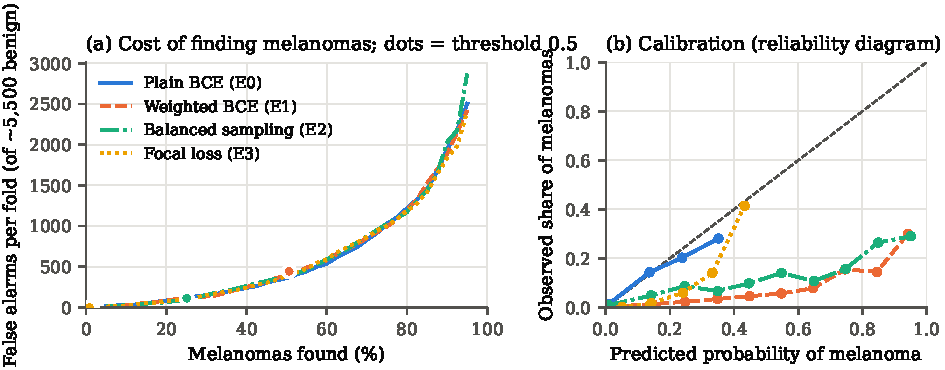
\includegraphics[width=\linewidth]{figures/fig1_tradeoff_reliability.pdf}
\caption{Plain BCE and three treatments, full fine-tuning, 5 held-out folds. (a) False alarms per fold needed to find a given share of melanomas: the four curves coincide, so no treatment separates better; the dots show where threshold 0.5 lands, which is all the treatments change. (b) Reliability diagrams: on the dashed line a score equals the observed share of melanomas. Only plain BCE stays on it.}
\label{fig:tradeoff}
\end{figure}

\subsection{Choosing the threshold}
\begin{notes}[~100 words, no exhibit]
  \item ``Best F1'' on inner validation (about 80 melanomas) transferred badly: plain BCE found between 15\% and 44\% of the melanomas on the held-out folds.
  \item ``Find 80\% on validation'' transferred well: 74--86\% for plain BCE, 73--82\% for the best extension model. We therefore used it for the test set.
\end{notes}

\subsection{Extension: more knowledge about melanoma helps}
\begin{notes}[~250 words; Figure~\ref{fig:steps}]
  \item Lead: the steps that change resolution or the ImageNet backbone did not help (384 px 0.163, 3/5; EfficientNet-B0 0.169, 2/5). EfficientNet memorised the training set (training AUROC 0.97 vs inner validation 0.85).
  \item The two steps that add knowledge about skin each helped on their own: PanDerm frozen 0.184 (4/5), ISIC 2019 on ResNet-18 0.206 (4/5); both lowered the price per melanoma from 5.1 to about 3.4 false alarms.
  \item Together they helped only when the backbone could adapt: frozen PanDerm + ISIC 2019 fell to 0.176 (3/5), fine-tuned PanDerm reached 0.264 (5/5) and fine-tuned PanDerm + ISIC 2019 \textbf{0.322} (5/5, and better than ISIC 2019 on ResNet-18 on all 5 folds). False alarms to find 80\% of melanomas: 757 per fold vs 1,219 for plain BCE.
  \item Metadata added nothing (0.317, better than without on 2/5 folds).
  \item Leakage check: without the Queensland and Sydney images the best model still wins on all 5 folds (0.29--0.40 vs 0.10--0.24).
  \item Training length (Figure~\ref{fig:long}): with PanDerm's 50-epoch schedule (fold 0), inner validation peaked at epoch 10; from epoch 24 the network fitted its training images perfectly (AUROC 1.000) while validation fell. Held-out AUPRC at the selected epoch was 0.309, below the 8-epoch run (0.333). The run stopped after 29 epochs (Colab limit); the curves already answer the question.
\end{notes}

\begin{figure}[t]
\centering
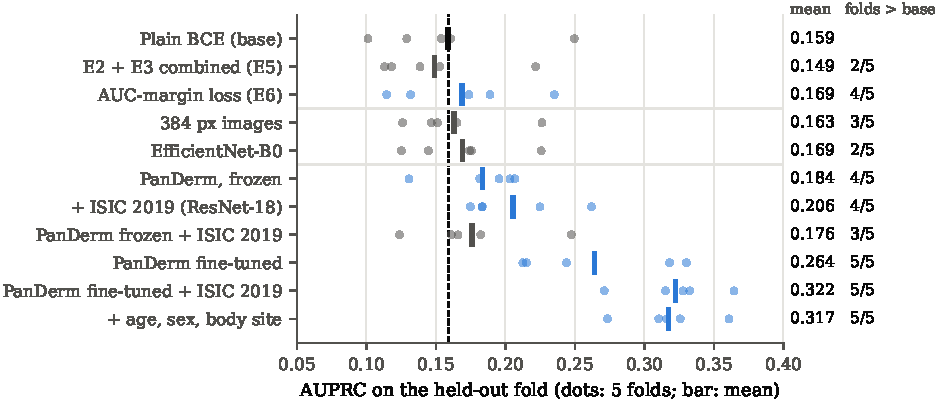
\includegraphics[width=\linewidth]{figures/fig2_steps.pdf}
\caption{AUPRC on the held-out folds for every treatment and extension step (dots: the 5 folds; bar: mean; dashed line: plain BCE). Blue steps pass the rule (mean above plain BCE and better on at least 4 of 5 folds); right: mean and number of folds better than plain BCE. Grey lines separate treatments, ImageNet changes and skin-specific changes.}
\label{fig:steps}
\end{figure}

\begin{figure}[t]
\centering
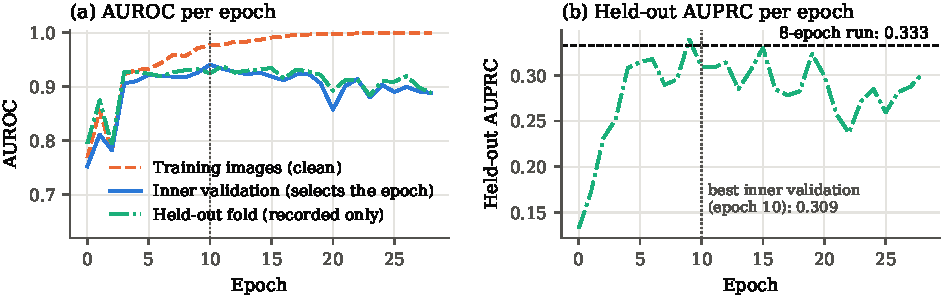
\includegraphics[width=\linewidth]{figures/fig3_long_training.pdf}
\caption{PanDerm fine-tuned + ISIC 2019 with the authors' 50-epoch schedule, fold 0 (stopped by Colab after 29 epochs). (a) The training AUROC reaches 1.000 while inner validation and held-out AUROC fall: the network overfits. (b) The epoch selected on inner validation (dotted) gives a held-out AUPRC below that of our 8-epoch run (dashed). The held-out fold was recorded only, never used for selection.}
\label{fig:long}
\end{figure}

\subsection{Locked test set}
\begin{notes}[~150 words; Table~\ref{tab:test}, Figure~\ref{fig:test}]
  \item Lead: on the test set the best extension model reached AUPRC 0.291 [0.197, 0.394] vs 0.154 [0.092, 0.237] for plain BCE; paired difference +0.138 [+0.059, +0.218].
  \item At the pre-registered threshold: 71 of 82 melanomas found with 561 false alarms, vs 62 with 1,002 for plain BCE (44\% fewer false alarms, 9 more melanomas).
  \item AUC-margin loss: 0.187, paired difference +0.033 [+0.009, +0.067] -- small but consistent with the folds (+0.010).
  \item Validation vs test: plain BCE 0.159 vs 0.154; AUC-margin 0.169 vs 0.187; best model 0.322 vs 0.291 (lower, as expected after choosing the best of many steps on the same folds).
  \item Without Queensland/Sydney images: 0.320 vs 0.171 -- no sign that the gain comes from images PanDerm may have seen.
  \item Threshold transfer: aimed at 80\%, found 76\% / 74\% / 87\%.
\end{notes}

\begin{table}[t]
\centering
\caption{Locked test set, opened once (4,630 images, 82 melanomas, 309 patients). Brackets: 95\% confidence intervals from 2,000 bootstrap resamples over patients. Threshold fixed beforehand to find 80\% of melanomas in the out-of-fold predictions. Differences are paired against plain BCE.}
\label{tab:test}
\small
\begin{tabular}{@{}lcccccc@{}}
\toprule
Model & AUPRC & $\Delta$AUPRC vs E0 & AUROC & Found / 82 & False alarms & ECE \\
\midrule
Plain BCE (E0) & 0.154 [0.092, 0.237] & -- & 0.870 & 62 & 1,002 & \textbf{0.005} \\
AUC-margin loss (E6) & 0.187 [0.113, 0.289] & +0.033 [+0.009, +0.067] & 0.883 & 61 & 958 & 0.101 \\
PanDerm FT + ISIC 2019 & \textbf{0.291} [0.197, 0.394] & \textbf{+0.138} [+0.059, +0.218] & \textbf{0.936} & \textbf{71} & \textbf{561} & 0.008 \\
\bottomrule
\end{tabular}
\end{table}

\begin{figure}[t]
\centering
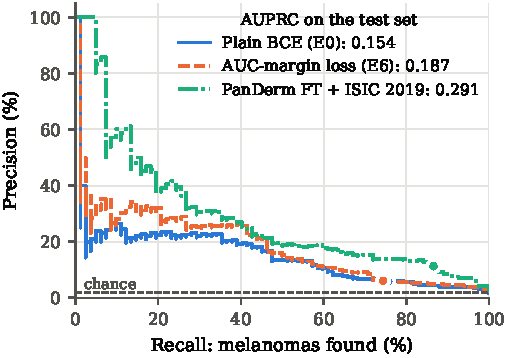
\includegraphics[width=0.55\linewidth]{figures/fig4_test_pr.pdf}
\caption{Precision--recall curves on the locked test set. Dots: the pre-registered threshold (aimed at 80\% recall). The extension model is above both ResNet-18 models at every recall; the dashed line is the 1.8\% chance level.}
\label{fig:test}
\end{figure}

% =============================================================================
\section{Discussion}
\label{sec:discussion}
\begin{notes}[450--550 words; explain WHY, with evidence; compare with related work]
  \item Why the treatments only move the threshold: they re-weight or repeat the \emph{same} ~400 training melanomas per fold; no new information enters. Evidence: identical cost curves (Fig.~\ref{fig:tradeoff}a), balanced sampling memorising its melanomas in 2--3 epochs. Agrees with Kang et al.~\cite{kang2020decoupling} (re-balancing acts on the classifier, not the features); unlike Buda et al.~\cite{buda2018systematic}, oversampling gave no gain once a threshold is tuned.
  \item Calibration: unlike Mukhoti et al.~\cite{mukhoti2020calibrating}, focal loss worsened calibration because our BCE baseline was not over-confident to begin with. Practical point: if a calibrated risk is needed, plain BCE + a chosen threshold is the better design.
  \item Why the AUC-margin loss helps a little: it is the only loss that targets the ranking itself; gain +0.01 (folds) / +0.03 (test), an order of magnitude below the data and backbone effects.
  \item Why the extension works: the limit is the number of melanomas the network can learn from. Evidence: EfficientNet memorised; ISIC 2019 brings ~11$\times$ more melanomas and narrowed the train/validation gap (0.925 vs 0.897); PanDerm brings features learnt from 2M skin images. They combine only when the backbone is fine-tuned (frozen: a single linear layer dominated by ISIC 2019's melanomas, which come from other clinics and cameras).
  \item Comparison with the winners~\cite{ha2020identifying}: they also trained on ISIC 2019 and used large EfficientNets; their ensemble (AUROC about 0.95 on the challenge's own test set) is not directly comparable to ours (different test set, ensemble of 18 large models, AUROC rather than AUPRC). Our 384 px and EfficientNet-B0 steps suggest their gains need the extra data and model size together.
  \item Limitations (about the experiment, not the tools): one seed per run (fold spread as uncertainty; test CIs do not include training noise); settings tuned on fold 0, whose inner validation overlaps other runs' held-out folds (can only favour the treatments); many extension steps chosen on the same folds (optimism, seen as 0.322 $\to$ 0.291); possible PanDerm pretraining overlap (checked, gain holds without Australian images); 32 identical image pairs across our own splits (all benign); the final models were retrained on all dev images, which shifted the threshold (87\% found instead of 80\%); 50-epoch run only on one fold and stopped at 29 epochs.
\end{notes}

% =============================================================================
\section{Conclusion}
\label{sec:conclusion}
\begin{notes}[100--150 words; do not copy the abstract]
  \item Answer the question in the introduction's words: no -- weighted loss, balanced sampling and focal loss moved the threshold and worsened calibration without improving separation; a ranking (AUC-margin) loss gave a small, consistent gain.
  \item What did help, with the number: real extra melanomas and skin-specific pretraining, combined with full fine-tuning: test AUPRC 0.291 vs 0.154.
  \item Practical message: tune the threshold (find-X\% rule), keep plain BCE for calibration, spend effort on data and features.
  \item One or two concrete next steps: repeat with several seeds; fine-tune PanDerm with the AUC-margin loss; evaluate on an external test set.
\end{notes}

% =============================================================================
\section*{Code and data}
Code: \url{https://github.com/Mikkelflassen/dlvr-g10}. Data: ISIC 2020 and ISIC 2019, resized by C.~Deotte on Kaggle (\texttt{cdeotte/jpeg-melanoma-256x256}, \texttt{cdeotte/jpeg-isic2019-256x256}); download instructions in the repository README. The test-set protocol (\texttt{docs/test\_protocol.md}) was committed before the test set was opened.

\begin{notes}[before hand-in]
  \item Attach the AU AI declaration; add the AI / source comments in the code (decided 17 Oct).
  \item Ask the TA whether references count toward the 6--8 pages.
  \item Check the two CHECK entries in references.bib.
\end{notes}

\bibliographystyle{unsrtnat}
\bibliography{references}

\end{document}
